\section{Results}
\label{sec:results}

\subsection{Part 1}

Table~\ref{tab:p1models} compares the reason-labeling methods. The mixture used
on its own is easily the weakest, and the obvious supervised default---one
separate classifier per reason---is beaten by the single balanced model over all
five. Letting the model teach itself adds the biggest single gain, and feeding the
mixture into that step gives the best validation score and the best
cross-validated score of anything we tried.

\begin{table}[t]
\centering\small
\begin{tabular*}{\columnwidth}{@{\extracolsep{\fill}}cccc@{}}
\toprule
\multicolumn{2}{c}{Validation} & \multicolumn{2}{c}{Repeated CV} \\
\cmidrule(lr){1-2}\cmidrule(lr){3-4}
samp.\ F1 & macro F1 & samp.\ F1 & macro F1 \\
\midrule
\multicolumn{4}{@{}l@{}}{\textit{One-vs-rest LR ($C{=}1$)}} \\
0.868 & 0.706 & 0.898 & 0.797 \\
\addlinespace
\multicolumn{4}{@{}l@{}}{\textit{$k$NN cosine ($k{=}10$)}} \\
0.872 & 0.607 & 0.881 & 0.734 \\
\addlinespace
\multicolumn{4}{@{}l@{}}{\textit{GMM-30 cluster-then-label}} \\
0.780 & 0.570 & 0.819 & 0.640 \\
\addlinespace
\multicolumn{4}{@{}l@{}}{\textit{Multinomial LR, unbalanced}} \\
0.850 & 0.677 & 0.894 & 0.765 \\
\addlinespace
\multicolumn{4}{@{}l@{}}{\textit{Balanced multinomial LR $+$ $k$NN}} \\
0.885 & 0.724 & 0.898 & 0.800 \\
\addlinespace
\multicolumn{4}{@{}l@{}}{\textit{Self-training, no GMM}} \\
0.889 & 0.723 & 0.913 & 0.805 \\
\addlinespace
\multicolumn{4}{@{}l@{}}{\textbf{Final: GMM-assisted self-training}} \\
\textbf{0.893} & 0.714 & \textbf{0.914} & \textbf{0.814} \\
\bottomrule
\end{tabular*}
\caption{Part~1 model comparison; each model's name heads its row of scores.
Validation is the 78 labeled trials; repeated CV is 8 repeats of 5-fold CV over
all 235 labeled trials.}
\label{tab:p1models}
\end{table}

Table~\ref{tab:p1ablation} adds each optional feature block to that model. Every
one of them leaves the validation score the same or worse, and none shifts the
cross-validated score by more than 0.013 either way, which is within the noise we
see between repeats. We therefore submitted the embeddings-only model;
Section~\ref{sec:discussion} explains why the extra features do not help.

\begin{table}[t]
\centering\small
\begin{tabular*}{\columnwidth}{@{\extracolsep{\fill}}cccc@{}}
\toprule
\multicolumn{2}{c}{Validation} & \multicolumn{2}{c}{Repeated CV} \\
\cmidrule(lr){1-2}\cmidrule(lr){3-4}
samp.\ F1 & macro F1 & samp.\ F1 & macro F1 \\
\midrule
\multicolumn{4}{@{}l@{}}{\textbf{Embeddings only}} \\
\textbf{0.893} & \textbf{0.714} & 0.914 & 0.814 \\
\addlinespace
\multicolumn{4}{@{}l@{}}{\textit{$+$ \texttt{start\_year}}} \\
0.891 & 0.711 & 0.912 & 0.807 \\
\addlinespace
\multicolumn{4}{@{}l@{}}{\textit{$+$ criteria TF-IDF (SVD 50)}} \\
0.876 & 0.709 & 0.913 & 0.801 \\
\addlinespace
\multicolumn{4}{@{}l@{}}{\textit{$+$ diseases TF-IDF (SVD 20)}} \\
0.876 & 0.696 & 0.914 & 0.806 \\
\addlinespace
\multicolumn{4}{@{}l@{}}{\textit{$+$ Morgan fingerprints (SVD 20)}} \\
0.889 & 0.719 & 0.918 & 0.815 \\
\bottomrule
\end{tabular*}
\caption{Part~1 feature ablation, final model; each feature set heads its row of
scores. No added block improves validation sample-F1.}
\label{tab:p1ablation}
\end{table}

Broken down by reason, validation F1 is 0.947 for Safety, 0.400 for Funding,
0.741 for Efficacy, 0.980 for Recruitment and 0.500 for Other, averaging 0.893
across trials and 0.714 across the five reasons. The two common reasons are
handled well and the two rarest are not, which we return to in
Section~\ref{sec:discussion}. Trained on the 157 labeled trials the model accepted
985 of its own pseudo-labels; refit on all 235 labeled trials it scores
\textbf{0.89423} on the Kaggle test set. Figure~\ref{fig:p1freq} shows what it
predicts for the later test trials: more Safety than in the labeled trials (0.173
against 0.106) and less Recruitment (0.587 against 0.643), which is the shift the
task description leads us to expect.

\begin{figure}[t]
\centering
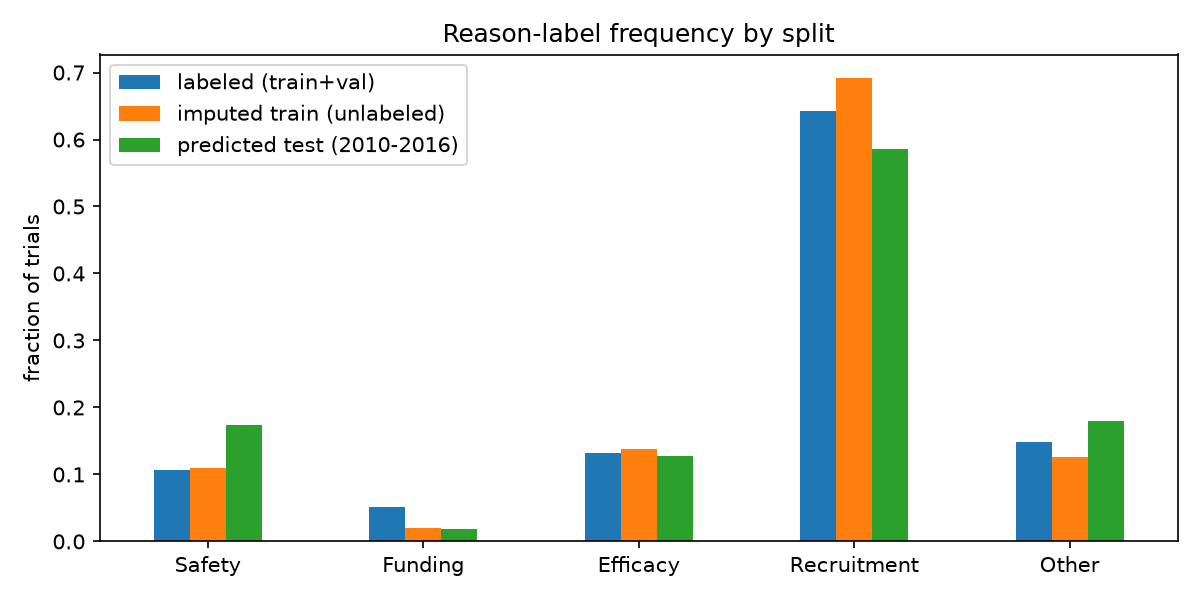
\includegraphics[width=0.95\linewidth]{part1_label_frequency.png}
\caption{Reason-label frequency across the labeled trials, the imputed unlabeled
training trials, and the predicted 2010--2016 test trials.}
\label{fig:p1freq}
\end{figure}

\subsection{Part 2}

Table~\ref{tab:p2val} reports the validation results for each phase. Naive Bayes
ranks trials about as well as logistic regression does, but states its answers far
too confidently, so its log loss of 2.646 is hopeless for a competition scored on
log loss. The stack improves both log loss and PR-AUC in every phase. Adding
recency weights improves log loss further and wins back the F1 that the plain
stack had given up.

\begin{table}[t]
\centering\small
\setlength{\tabcolsep}{3.5pt}
\begin{tabular}{llcccc}
\toprule
Phase & Metric & MNB & Base LR & Stack & $+$Rec \\
\midrule
\multirow{4}{*}{I}
 & F1       & 0.737 & 0.774 & 0.730 & \textbf{0.793} \\
 & ROC-AUC  & 0.717 & 0.780 & 0.772 & \textbf{0.793} \\
 & PR-AUC   & 0.733 & 0.809 & 0.816 & \textbf{0.828} \\
 & log loss & 2.684 & 0.609 & 0.570 & \textbf{0.557} \\
\midrule
\multirow{4}{*}{II}
 & F1       & 0.645 & 0.631 & \textbf{0.661} & 0.648 \\
 & ROC-AUC  & 0.694 & 0.729 & 0.749 & \textbf{0.754} \\
 & PR-AUC   & 0.623 & 0.711 & 0.733 & \textbf{0.735} \\
 & log loss & 2.945 & 0.610 & \textbf{0.591} & 0.593 \\
\midrule
\multirow{4}{*}{III}
 & F1       & 0.796 & 0.813 & 0.817 & \textbf{0.824} \\
 & ROC-AUC  & 0.699 & 0.764 & \textbf{0.787} & \textbf{0.787} \\
 & PR-AUC   & 0.783 & 0.868 & \textbf{0.883} & 0.881 \\
 & log loss & 2.308 & 0.553 & \textbf{0.516} & 0.518 \\
\midrule
\multirow{4}{*}{mean}
 & F1       & 0.726 & 0.739 & 0.736 & \textbf{0.755} \\
 & ROC-AUC  & 0.703 & 0.758 & 0.769 & \textbf{0.778} \\
 & PR-AUC   & 0.713 & 0.796 & 0.810 & \textbf{0.814} \\
 & log loss & 2.646 & 0.591 & 0.559 & \textbf{0.556} \\
\bottomrule
\end{tabular}
\caption{Part~2 validation metrics by phase. Columns are the per-phase
multinomial naive Bayes (MNB), the per-phase criteria-only logistic regression
(Base LR), the stacked ensemble (Stack) and the recency-weighted stack
($+$Rec, $\tau{=}3$). F1 uses a 0.5 threshold; ROC-AUC, PR-AUC and log loss use
predicted probabilities, with $\text{label}=1$ positive. Best value per row in
bold.}
\label{tab:p2val}
\end{table}

The time-ordered holdouts in Table~\ref{tab:p2holdout} ask the question that
matters for the leaderboard: does the ranking still hold when the trials being
scored are later than the trials used to train? It does. Training on everything up
to 2009 and scoring 2010--2013, the stack cuts log loss from 0.5879 to 0.5514, and
recency weighting takes it to 0.5475. On the harder split, training to 2011 and
scoring 2012--2013, the same three steps give 0.5192, then 0.4657, then 0.4553, so
the gap grows as the evaluation moves further from the training years.

\begin{table}[t]
\centering\small
\setlength{\tabcolsep}{3.5pt}
\begin{tabular}{llcccc}
\toprule
Fit cut & Metric & MNB & Base LR & Stack & $+$Rec \\
\midrule
\multirow{4}{*}{$\leq$2009}
 & F1       & 0.8083 & 0.8051 & 0.8090 & \textbf{0.8094} \\
 & ROC-AUC  & 0.6295 & 0.6943 & 0.7248 & \textbf{0.7311} \\
 & PR-AUC   & 0.7301 & 0.7847 & 0.8183 & \textbf{0.8205} \\
 & log loss & 2.4794 & 0.5879 & 0.5514 & \textbf{0.5475} \\
\midrule
\multirow{4}{*}{$\leq$2011}
 & F1       & 0.8576 & 0.8654 & 0.8697 & \textbf{0.8758} \\
 & ROC-AUC  & 0.5970 & 0.7042 & 0.7539 & \textbf{0.7604} \\
 & PR-AUC   & 0.7740 & 0.8290 & 0.8850 & \textbf{0.8865} \\
 & log loss & 2.0120 & 0.5192 & 0.4657 & \textbf{0.4553} \\
\bottomrule
\end{tabular}
\caption{Part~2 time-based holdouts, mean over phases; columns as in
Table~\ref{tab:p2val}. ``Fit cut'' is the last start year in the fitting set: the
2009 cut is evaluated on 2010--2013 and the 2011 cut on 2012--2013. These mimic the later start years of the test set and were used to
select $\tau$. Best value per row in bold.}
\label{tab:p2holdout}
\end{table}

On the Kaggle test set the final submission scores \textbf{0.58688} mean log
loss, against 0.556 on validation---a gap we return to in
Section~\ref{sec:discussion}.

\subsection{Error analysis across reason categories}

Table~\ref{tab:p2errors} and Figure~\ref{fig:p2err} break the failed validation
trials down by phase and stopping reason. Two patterns hold up. First, the
classifier is far more likely to mistake a failed Phase~III trial for a success
(0.57 to 1.00 for the baseline) than a failed Phase~II one (0.00 to 0.38), even
though Phase~III has more training data than Phase~I. Second, the groups large
enough to trust---Phase~II Recruitment with 87 trials, and the three
no-recorded-reason groups with 28, 144 and 82---improve at every step from the
baseline to the stack to the recency-weighted stack. The Phase~I no-reason group
drops from 0.643 to 0.321, less than half its original error rate.

\begin{figure*}[t]
\centering
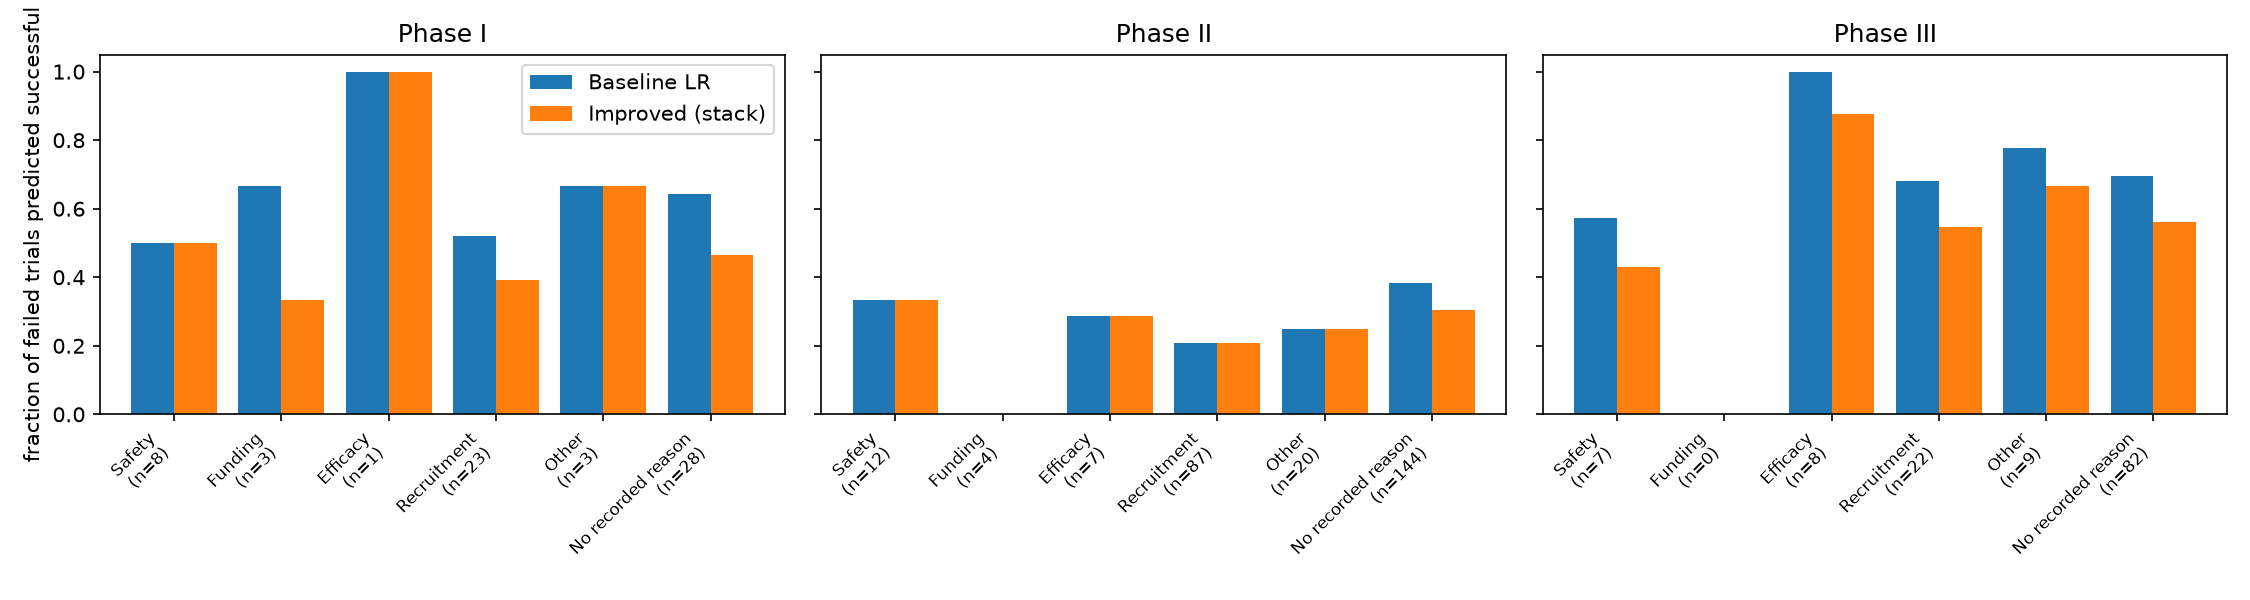
\includegraphics[width=\textwidth]{part2_error_by_reason.png}
\caption{Fraction of failed validation trials incorrectly predicted successful,
by phase and stopping reason, for the criteria-only baseline and the stacked
ensemble. Group sizes are given in the tick labels.}
\label{fig:p2err}
\end{figure*}

\begin{table*}[t]
\centering\small
\begin{tabular}{llccccccc}
\toprule
& & \multicolumn{3}{c}{Group composition} & & \multicolumn{3}{c}{Fraction predicted successful} \\
\cmidrule(lr){3-5}\cmidrule(lr){7-9}
Phase & Reason & $n$ trials & $n$ true & $n$ predicted & & Baseline LR & Improved & Final \\
\midrule
I & Safety             &  8 &  1 &  7 & &  0.500 & 0.500 & 0.375 \\
I & Funding            &  3 &  1 &  2 & &  0.667 & 0.333 & 0.000 \\
I & Efficacy           &  1 &  0 &  1 & &  1.000 & 1.000 & 0.000 \\
I & Recruitment        & 23 &  2 & 21 & &  0.522 & 0.391 & 0.174 \\
I & Other              &  3 &  0 &  3 & &  0.667 & 0.667 & 0.667 \\
I & No recorded reason & 28 &  0 &  0 & &  0.643 & 0.464 & 0.321 \\
\midrule
II & Safety             &  12 &  1 & 11 & & 0.333 & 0.333 & 0.250 \\
II & Funding            &   4 &  1 &  3 & & 0.000 & 0.000 & 0.000 \\
II & Efficacy           &   7 &  0 &  7 & & 0.286 & 0.286 & 0.286 \\
II & Recruitment        &  87 & 12 & 75 & & 0.207 & 0.207 & 0.149 \\
II & Other              &  20 &  3 & 17 & & 0.250 & 0.250 & 0.250 \\
II & No recorded reason & 144 &  0 &  0 & & 0.382 & 0.306 & 0.250 \\
\midrule
III & Safety             &  7 & 1 &  6 & & 0.571 & 0.429 & 0.429 \\
III & Funding            &  0 & 0 &  0 & & ---   & ---   & ---   \\
III & Efficacy           &  8 & 0 &  8 & & 1.000 & 0.875 & 1.000 \\
III & Recruitment        & 22 & 5 & 17 & & 0.682 & 0.545 & 0.455 \\
III & Other              &  9 & 2 &  7 & & 0.778 & 0.667 & 0.556 \\
III & No recorded reason & 82 & 0 &  0 & & 0.695 & 0.561 & 0.585 \\
\bottomrule
\end{tabular}
\caption{Error rates on the 452 failed validation trials, by phase and stopping
reason. ``$n$ true'' counts trials whose reason labels are ground truth from
Part~1; ``$n$ predicted'' counts trials whose reason labels are Part~1 model
predictions. A trial with several reasons appears in each of its reason rows, so
columns do not sum to the phase total.}
\label{tab:p2errors}
\end{table*}
